We were mainly interested in answering two questions:

\begin{enumerate}

  \item how far in the future can our system predict well?

  \item how does the knowledge of the grasped object affect the error?

\end{enumerate}

In order to answer the first question, we have checked how the error
on regression changes as the \emph{blind fraction} $0 \leq B \leq 1$
of the grasp increases from $0.1$ to $0.5$. The blind fraction
indicates what percentage of the grasp, from the contact point
backwards, is hidden to the system. It was expected that larger values
of $B$ would smoothly lead to larger errors. Figure
\ref{fig:B_example} shows a typical situation.

\begin{figure}[htbp]
  \begin{center}
    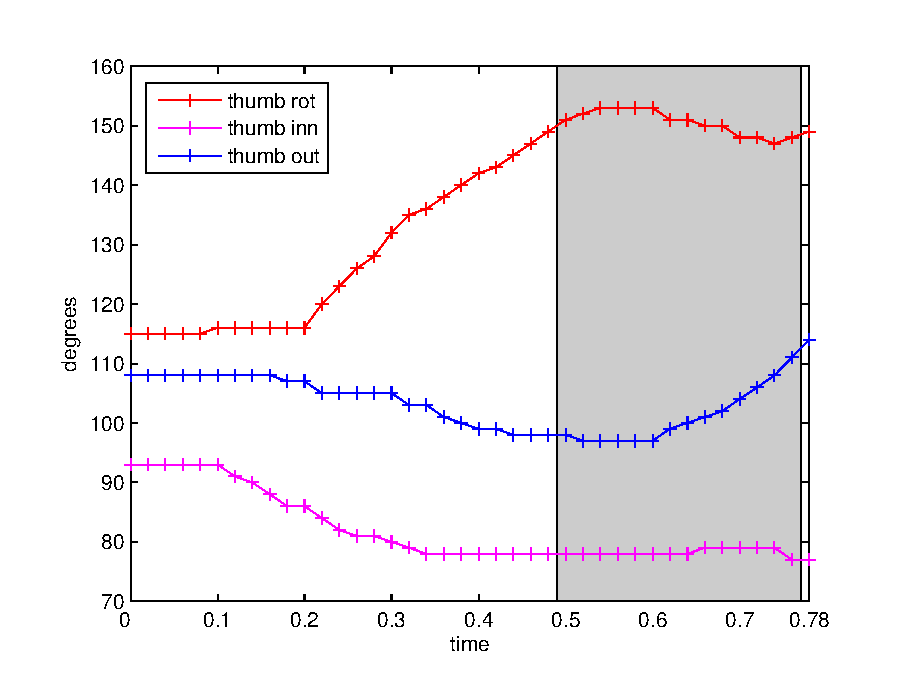
\includegraphics[width=0.5\linewidth]{B_example.eps}
    \caption{The blind window (the grey zone in the Figure) indicates
    what fraction of each grasp, from the contact point backwards, is
    hidden to the SVM. The data shown is a typical trajectory of the
    thumb (rotation, inner phalanx, outer phalanx) during a grasp. In
    this case the grasp lasts $0.78$ seconds and $B=0.375$. The last
    sample (for $t=0.78$) is the target value.}
    \label{fig:B_example}
  \end{center}
\end{figure}

This procedure was repeated independently for each single sensor. The
errors for each sensor were then grouped and averaged accordingly to
their measurement unit and meaning: the position of the hand ($3$
sensors, the $x,y,z$ from the FoB), the hand orientation ($3$ sensors,
the azimuth, elevation and roll from the FoB), and the posture of the
hand ($22$ sensors, the joint positions from the
CyberGlove). According to the device resolutions detailed in the
previous Section, we set $\epsilon$ to $0.1$ inches for the hand
position, $0.5$ degrees for the hand orientation and $1$ degree for
the hand posture.

In order to answer the second question, we first compared the error
obtained as described above using all sessions for each single object,
so to obtain an estimate of how complex it is to approximate the grasp
for the can, roll and mug, unbiased by the differences among the
subjects. Subsequently we averaged these three errors and compared the
average with the overall error, obtained by joining \emph{all}
sessions together. Figure \ref{fig:err_all} shows the experimental
results.

\begin{figure}[htbp]
  \begin{center}
    \begin{tabular}{cc}
      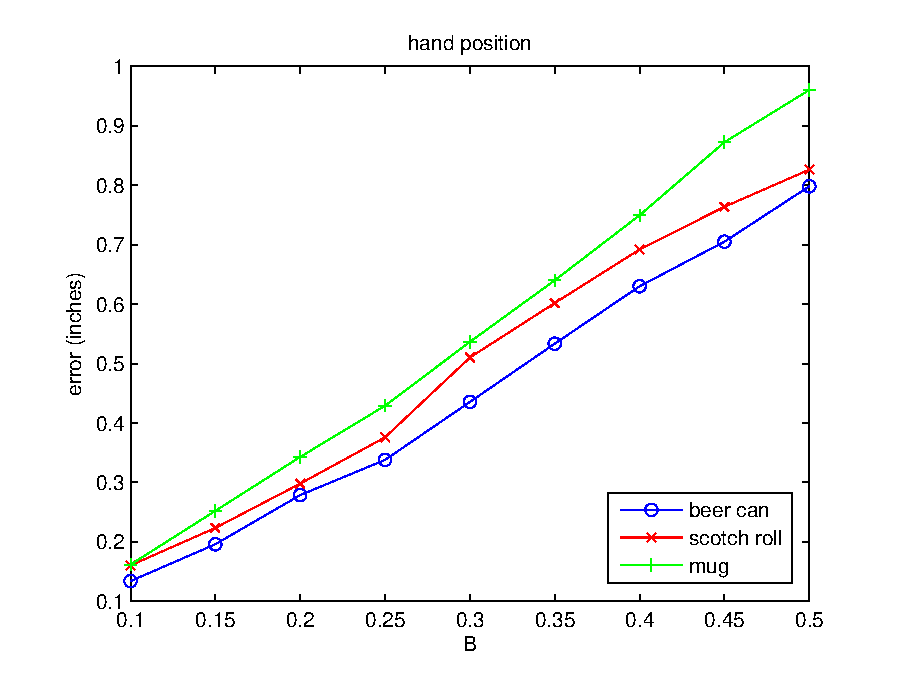
\includegraphics[width=0.45\textwidth]{error_pos.eps} &
      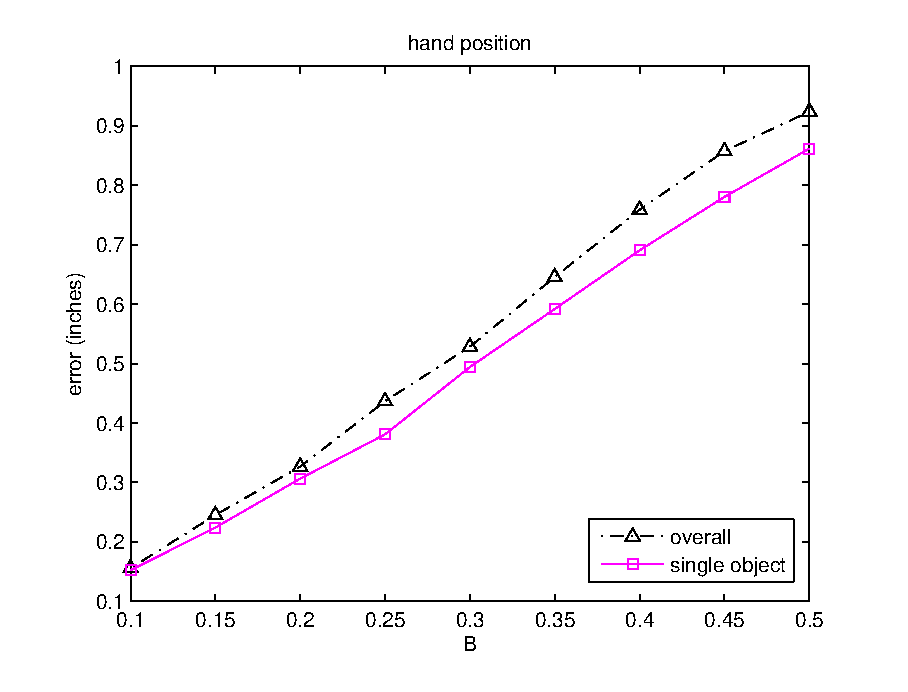
\includegraphics[width=0.45\textwidth]{error_cmp_pos.eps} \\
      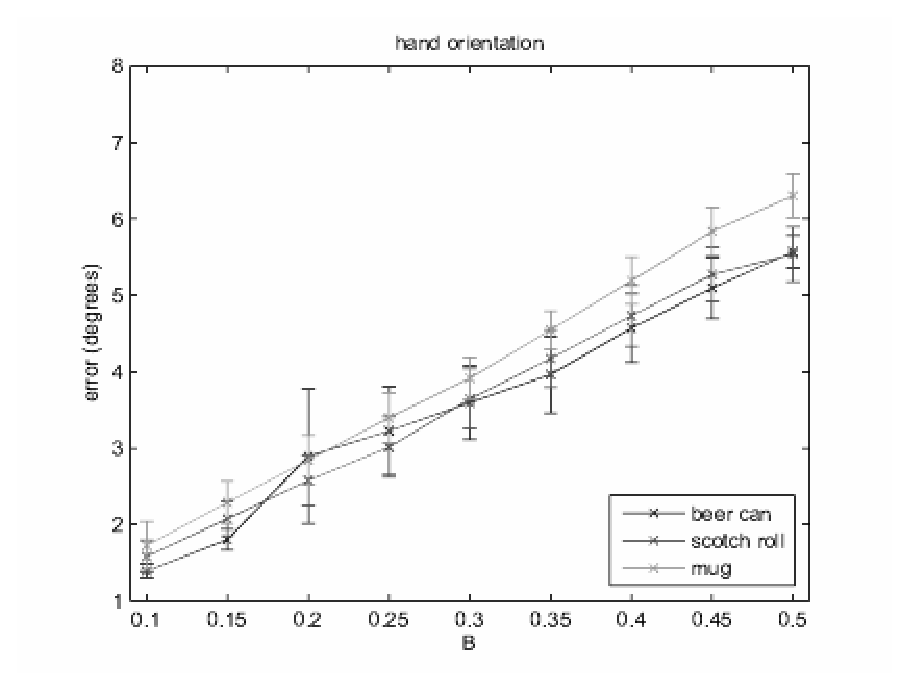
\includegraphics[width=0.45\textwidth]{error_ori.eps} &
      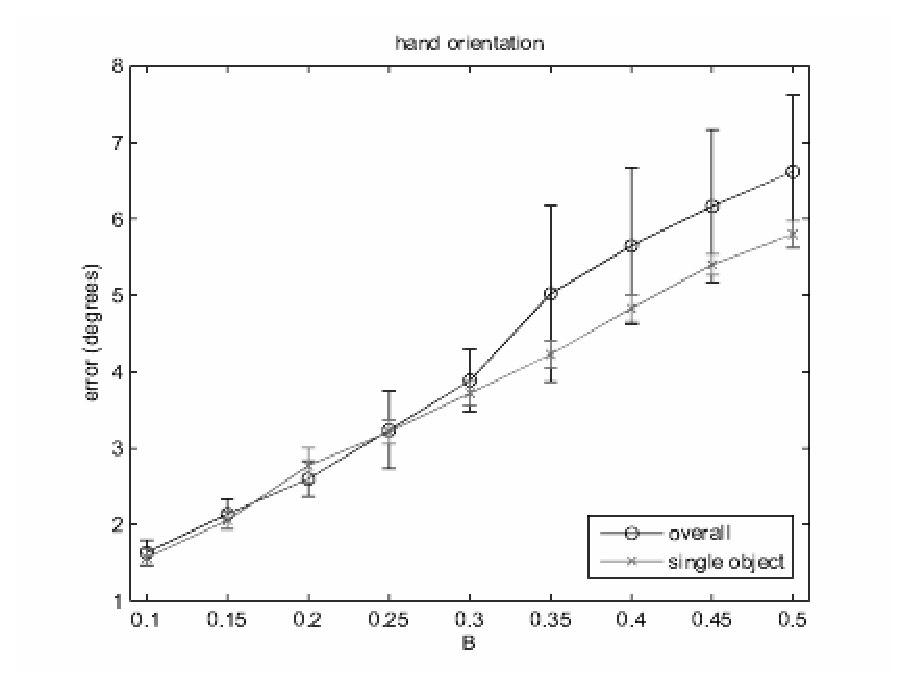
\includegraphics[width=0.45\textwidth]{error_cmp_ori.eps} \\
      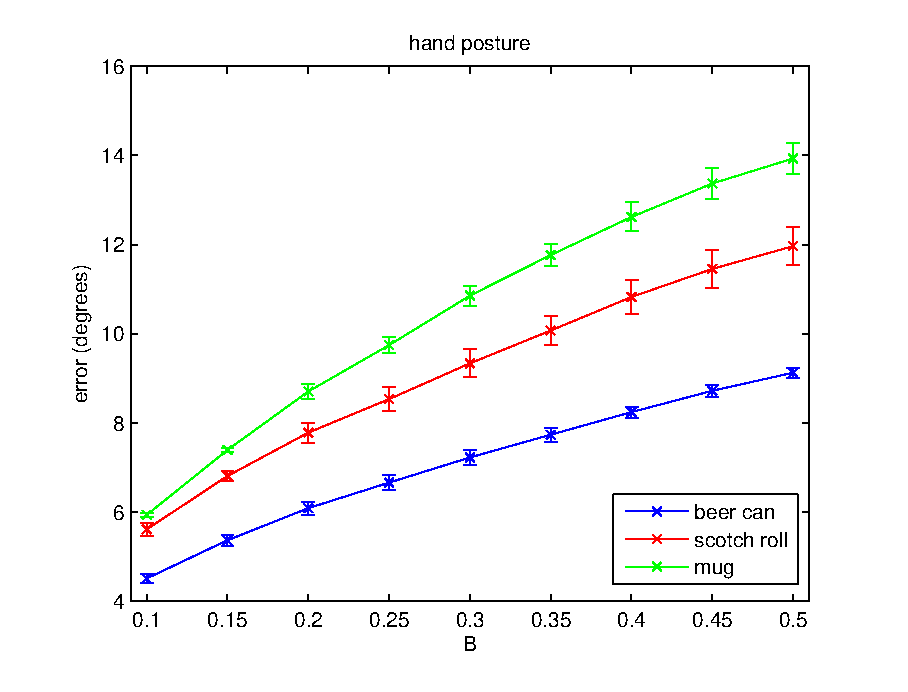
\includegraphics[width=0.45\textwidth]{error_pst.eps} &
      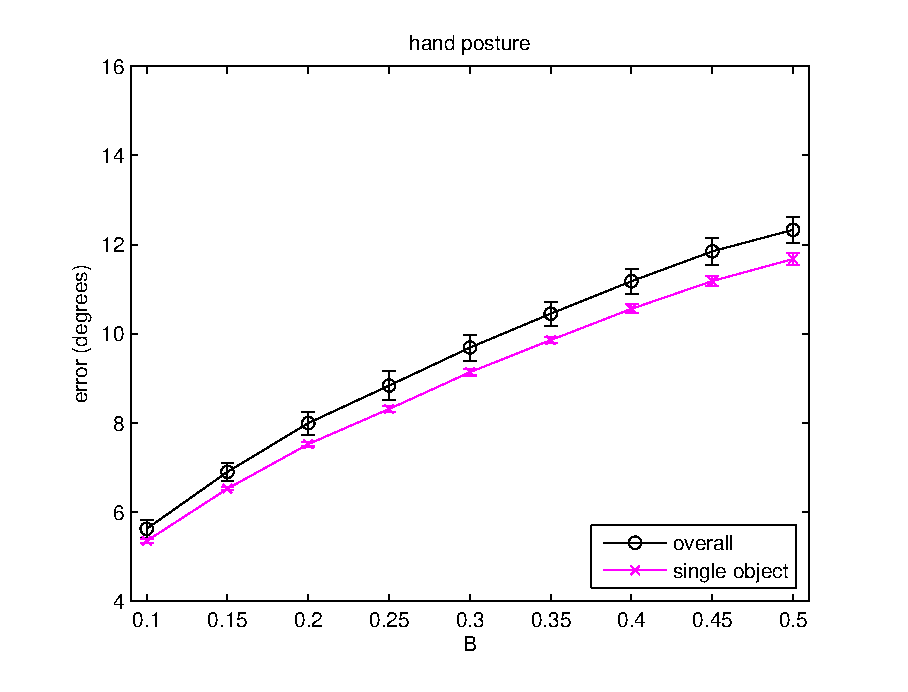
\includegraphics[width=0.45\textwidth]{error_cmp_pst.eps} \\
    \end{tabular}
    \caption{Regression results as the blind fraction $B$ increases
    from $0.1$ to $0.5$. In each row, representing a different set of
    sensors (in turn, hand position, orientation and posture), the
    left-hand side pictures compare the errors on different objects,
    while the right-hand side pictures comapre the average error on
    single objects and the overall error.}
    \label{fig:err_all}
  \end{center}
\end{figure}

Consider Figure \ref{fig:err_all}, left column: as one can see, as far
as the hand position and orientation are concerned, the three objects
show a comparable error. On the other hand, there is a precise ranking
in the hand posture regression: the mug is more difficult than the
scotch roll, which is in turn harder than the beer can. This is
intuitively sensible, since it is possible to grasp the scotch roll in
more ways than the can, and it is possible to grasp the mug in even
more ways (especially, using the handle).

Since the hand position sensors have a resolution of $0.1$ inches, a
resonable error seems to be about $0.5$ inches. This is on average
attained for $B=0.3$. Since the average grasp lasts on average $0.62$
seconds, we can say that the system can predict reasonably well
something less than $200$ milliseconds before the grasp what the hand
position will be. Similar considerations lead us to say that the
system is able to predict the hand orientation $120$ milliseconds
before the grasp with an error of about $2.5$ degrees. The hand
posture requires a slightly more careful study: since the maximum
noise on the CyberGlove sensors has been experimentally determined to
be $3$ degrees \cite{212431}, it seems reasonable to take half this
value as a minimal starting point. A five-fold error is then attained
at $B=0.15$ ($9$ milliseconds before the grasp) for the mug and the
scotch roll, and $B=0.3$ ($200$ milliseconds) for the can. This
anwsers the first question.

As far as the second question is concerned, consider Figure
\ref{fig:err_all}, right column: the average error attained on the
single objects is always consistently smaller than that attained on
the overall sequence. A further analysis of $C$ and $\gamma$, and the
number of support vectors retained by the machines, which indicates
``how hard'' the problems are, reveals that the computational
complexity of the tasks is comparable. The analysis of single objects
(sum over the three machines) requires about $1\%$ more support
vectors than the overall analysis. For each single-object machine, the
number of sample considered is about one third of the overall machine,
with $C$ being on average smaller. This indicates that the machines
trained on single objects are significantly faster than the one
trained on the overall sequence, while attaining a better accuracy.

Summing up, if the problem is split into subproblems, each one
regarding a single object, performances are better and the total
computational complexity remains roughly the same.
